\section{Spørgsmål 6}

% Hvad er Relationel Algebra (RA)? Kom herunder ind på: relation, tuple, set og operatorer (select, projection, join...) samt RA' betydningen for opbygningen af  SQL (Structured Querry Language) erklæringer

\subsection{Fokuspunkter}
\begin{itemize}
	\item Hvad er Relationel Algebra (RA)?
	\begin{itemize}
		\item Kom herunder ind på: relation, tuple, set og operatorer (select, projection, join...).
	\end{itemize}
	\item Samt RA' betydningen for opbygningen af  SQL (Structured Querry Language) erklæringer.
\end{itemize}

\subsection{Litteratur}
\begin{itemize}
	
%	\item Fra teori: Database Modeling and Design. Logical Design 5'th Ed.
%	\begin{itemize}
%		\item Ch. 1 (p1 - 11)
%		\item Ch. 2 (p13 - 34)
%		\item Ch. 3 (p35 - 53)
%		\item Ch. 4 (p55 - 84)
%	\end{itemize}
	
	\item Fra Database eLearning: \url{http://db.grussell.org/index.html}.
	\begin{itemize}
		\item Ralational Algebra.
		\begin{itemize}
			\item Introduction to Relational Algebra.
			\item Algebraic format Relational Algebra.
		\end{itemize}
	\end{itemize}
	
%	\item Fra wikipedia:
%	\begin{itemize}
%		\item 
%	\end{itemize}
%	
%	\item Fra Agile Data Home Page:
%	\begin{itemize}
%		\item 
%	\end{itemize}
\end{itemize}

\newpage

% must
\subsection{Hvad er Relationel Algebra (RA)?}

\textit{"There must be a set of rules which state how the database system will behave. For instance, somewhere in the DBMS\footnote{Database management system.} must be a set of statements which indicate, when someone inserts data into a relation, it has the effect which is expected. One way to specify this is to write an `essay' as to how the DBMS will operate, but words are imprecise and open to interpretation. Instead, relational databases are usually defined using Relational Algebra."}\\

Med andre ord så er RA \textbf{en entydig måde at beskrive en database's opførsel}: 

\begin{itemize}
	\item The formal description of how a relational database operates.
	\item An interface to the data stored in the database itself.
	\item The mathematics which underpin SQL operations.
\end{itemize}

Videre så forklare teksten: \textit{"Operators in relational algebra are not the same as SQL operators, even if they have the same name. For example, the SELECT statement exists in SQL, and in RA. These two uses of SELECT are not the same. The DBMS takes whatever SQL statements the user types and translate them into RA operations before applying them to the database."}

% must
\subsubsection{Kom herunder ind på: relation, tuple, set og operatorer (select, projection, join...)}

\paragraph{Relation}
Et set af tupler.

\paragraph{Tuple}
En samling af attributter som beskriver \textit{"some real world entity"}.

\paragraph{Set}


\paragraph{Operatorer}

ælkjælkj ælkdj fgsælkdfsj gæodsfijgæ osdifj gpæoijg sdæ.

\begin{figure}[H]
	\centering
	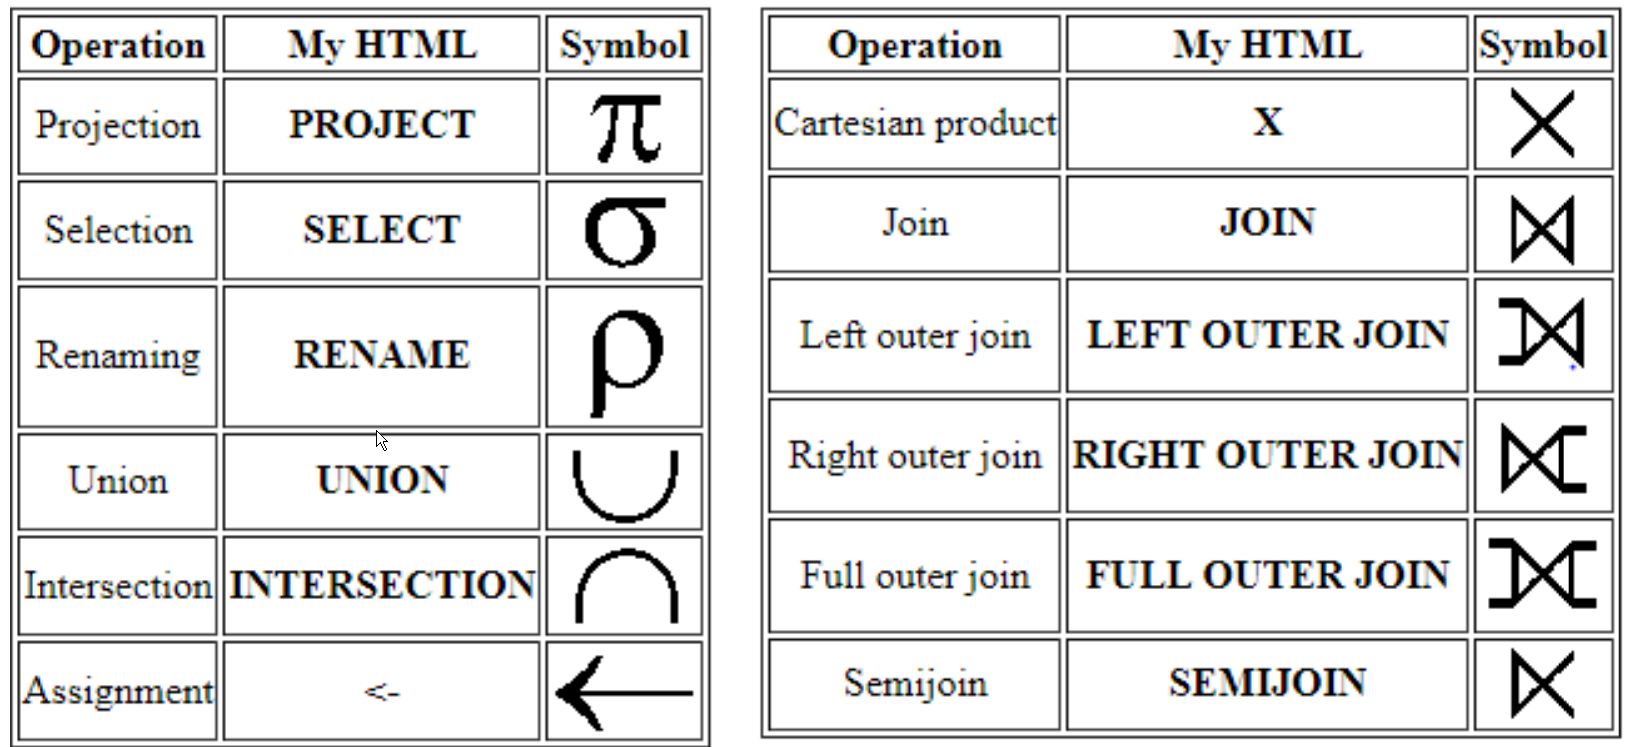
\includegraphics[width=\linewidth]{figs/spm6/operators}
	\caption{Forskellige operatore i RA.}
	\label{fig:operators}
\end{figure}


% must
\subsubsection{Samt RA' betydningen for opbygningen af  SQL (Structured Querry Language) erklæringer}



















